\section{一元函数积分学}

本节给出定积分的概念和意义。
定积分是一元函数积分学的目的,后续的牛顿莱布尼兹公式和不定积分是求解定积分的方法。

本节要点:
\begin{itemize}
    \item 理解定积分的概念和意义;
    \item 掌握用概念求解定积分。
\end{itemize}

%============================================================
\subsection{定积分的概念}

\begin{definition}[定积分]
设函数$f\left( x \right) $在$\left[ a,b \right] $上有界,将$\left[ a,b \right] $划分为$n$个小区间$a=x_0<x_1<x_2<...<x_{n-1}<x_n=b$,记每个小区间的长度$\Delta x_i=x_i-x_{i-1},i=1,2,...,n$,令最大长度$\lambda =\max \left\{ \Delta x_i \right\} $,在每个小区间$\left[ x_{i-1},x_i \right] $上任取一点$\xi _i\in \left[ x_{i-1},x_i \right] $,作和式$\sum_{i=1}^n{\left[ f\left( \xi _i \right) \cdot \Delta x_i \right]}$,若无论区间$\left[ a,b \right] $如何划分也无论点$\xi _i$如何选取,极限$\underset{\lambda \rightarrow 0}{\lim}\sum_{i=1}^n{\left[ f\left( \xi _i \right) \cdot \Delta x_i \right]}$存在且唯一,则称{\bf $f\left( x \right) $在$\left[ a,b \right] $上可积},该极限的值称为{\bf $f\left( x \right) $在$\left[ a,b \right] $上的定积分(definite integral)},记作$\int_a^b{f\left( x \right) dx}$,即:
\[
\int_a^b{f\left( x \right) dx}:=\underset{\lambda \rightarrow 0}{\lim}\sum_{i=1}^n{\left[ \xi _i\cdot \Delta x_i \right]}
\]
其中:
\begin{itemize}
    \item $x$:积分变量;
    \item $f\left( x \right) $:被积函数;
    \item $f\left( x \right) dx$:积分表达式,也称{\bf 微元};
    \item $a,b$:积分下限,积分上限;
    \item $\left[ a,b \right] $:积分区间。
\end{itemize}
\end{definition}

这个积分定义是黎曼(Riemann)给出的,通常称作{\bf 黎曼积分}。
黎曼积分存在的两个前提条件可以概括为闭区间和有限不连续。

\begin{tcolorbox}
黎曼可积的充要条件是勒贝格(Lebesgue)定理,即$f\left( x \right) $在$\left[ a,b \right] $上的不连续点组成的集合是一个零测度集。
如果不符合,则没有黎曼积分,需要扩充到勒贝格积分。
\end{tcolorbox}

注意,定积分概念里的两个“无关”:
\begin{itemize}
    \item 与区间划分方法无关,即$n$个小区间可以等分,也不可以不等分;
    \item 与区间点$\xi _i$的取法无关,即可以取在头、尾、中或者小区间内的任意一点。
\end{itemize}

\begin{tcolorbox}
一般的微积分教材里,将$\Delta x_i$称为“长度”。
但要特别注意,这个所谓的“长度”,是规定了方向的,是沿着{\it x}轴正方向,即$\Delta x_i=x_i-x_{i-1}$,不是$\Delta x_i=x_{i-1}-x_i$。
$\Delta x_i$必然是一个大于0的量。所以才有性质$\int_a^b{f\left( x \right) dx}=-\int_b^a{f\left( x \right) dx}$,细品!
\end{tcolorbox}

研究一函数在某一区间是否可积,关键在于判断和式极限
\[
\underset{\lambda \rightarrow 0}{\lim}\sum_{i=1}^n{\left[ f\left( \xi _i \right) \cdot \Delta x_i \right]}
\]
是否存在且唯一,步骤如下:
\begin{enumerate}
    \item 划分区间,通常等分;
    \item 取权重,通常取小区间的头或者尾;
    \item 求和式极限。
\end{enumerate}
所以定积分也是极限。
和求导一样,定积分也是对函数的一种运算,具体来说是对被积函数的一种运算,通过加权求和取极限这一过程得到另一个函数。
从集合角度,定积分是一个函数集合到另一个函数集合的映射。
这点在学习积分上限函数这个概念后细品!

%============================================================
\subsection{定积分的性质和定理}

区间性:
\begin{align*}
&a=b \quad \Rightarrow \quad \int_a^b{f\left( x \right) dx}=0 \\
&a\ne b \quad \Rightarrow \quad \int_a^b{f\left( x \right) dx}=-\int_b^a{f\left( x \right) dx}
\end{align*}

线性性:
\[
\int_a^b{\left[ mf\left( x \right) +ng\left( x \right) \right] dx}=m\int_a^b{f\left( x \right) dx}+n\int_a^b{g\left( x \right) dx}
\]

区间可加性:
\[
\int_a^b{f\left( x \right) dx}=\int_a^c{f\left( x \right) dx}+\int_c^b{f\left( x \right) dx}
\]

保号性:
\begin{align*}
&f\left( x \right) \geqslant 0 \quad \Rightarrow \quad \int_a^b{f\left( x \right) dx}\geqslant 0 \\
&f\left( x \right) \geqslant g\left( x \right) \quad \Rightarrow \quad \int_a^b{f\left( x \right) dx}\geqslant \int_a^b{g\left( x \right) dx}
\end{align*}

~

\begin{theorem}[连续可积定理]
$f\left( x \right) $在$\left[ a,b \right] $上连续$\Rightarrow f\left( x \right) $在$\left[ a,b \right] $上可积。
\end{theorem}

\begin{theorem}[有界可积定理]
$f\left( x \right) $在$\left[ a,b \right] $上有界,且只有有限个一类间断点$\Rightarrow f\left( x \right) $在$\left[ a,b \right] $上可积。
\end{theorem}

\begin{theorem}[估值定理]
设$M,m$分别是$f\left( x \right) $在$\left[ a,b \right] $上的最大值和最小值,则
\[
m\left( b-a \right) \leqslant \int_a^b{f\left( x \right) dx}\leqslant M\left( b-a \right)
\]
\end{theorem}

\begin{theorem}[积分中值定理]
若$f\left( x \right) $在$\left[ a,b \right] $上连续,则存在$\xi \in \left( a,b \right) $,使得
\[
\int_a^b{f\left( x \right) dx}=f\left( \xi \right) \left( b-a \right)
\]
\end{theorem}

估值定理和积分中值定理常用于定理的证明。
积分中值定理对应的微分中值定理中的拉格朗日定理,几何上表示必有矩形和曲边梯形面积相等,物理上必有均值点$\xi $及其均值$f\left( \xi \right) $。

\begin{tcolorbox}
细品后能发现,这些定理对曲线都要求不断。相比导数和微分,要求宽松了些。
\end{tcolorbox}

%============================================================
\subsection{定积分的代数意义}

在数学上,和式$\sum_{i=1}^n{\left[ f\left( \xi _i \right) \cdot \Delta x_i \right]}$可以看成加权和,每个累加项$\Delta x_i$加了权重$f\left( \xi _i \right) $后的代数和,整个和式也可以看成矩阵乘法:
\[
\sum_{i=1}^n{\left[ f\left( \xi _i \right) \cdot \Delta x_i \right]}=\left[ \begin{matrix}
	f\left( \xi _1 \right)&		f\left( \xi _2 \right)&		\cdots&		f\left( \xi _n \right)\\
\end{matrix} \right] \cdot \left[ \begin{array}{c}
	\Delta x_1\\
	\Delta x_2\\
	\vdots\\
	\Delta x_n\\
\end{array} \right]
\]
定积分就是当每个累加项都趋于无穷小,划分趋于无穷细、无穷多,情况下的这个代数和的极限。

\begin{tcolorbox}
从忽略高阶无穷小量的角度看,定积分的位置有点像微分。
\end{tcolorbox}

%============================================================
\subsection{定积分的几何意义}

考察曲线$y=f\left( x \right) $。
$f\left( \xi _i \right) \cdot \Delta x_i$是小区间的面积,和式$\sum_{i=1}^n{\left[ f\left( \xi _i \right) \cdot \Delta x_i \right]}$是所有小区间的面积的和,当小区间宽度越来越小时,和就越来越接近曲线下的面积。
当每个小区间的宽度都无穷小的时候,和式极限就是曲线下的面积。
所以几何上,定积分就是被积函数$y=f\left( x \right) $和{\it x}轴在积分区间$\left[ a,b \right] $里围成的面积。
\begin{figure}[h]
\centering
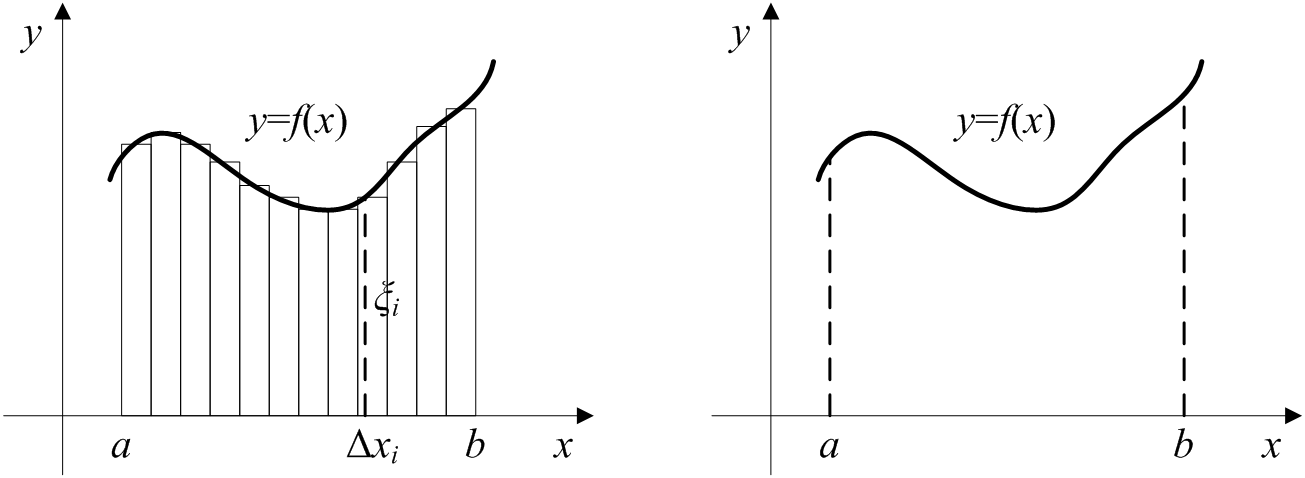
\includegraphics[height=3.5cm]{3.1.png}
\end{figure}

%============================================================
\subsection{定积分的物理意义}

物理量可以看成是很多分段小量的集合,每个小量又可以看成“加权小量”。
比方总路程$S$就可以看成很多分段$\Delta S$的累积,而$\Delta S$又是单位时间上平均速度的加权结果$\Delta S=\bar{v}\left( t \right) \cdot \Delta t$。
所以总路程为:
\[
S=\sum{\Delta S}=\sum{\left[ \bar{v}\left( t \right) \cdot \Delta t \right]}
\]
当单位时间$\Delta t\rightarrow 0$时,$\Delta t=dt$且有平均速度变成瞬时速度$\bar{v}\left( t \right) =v\left( t \right) $,有限段小路程变成无穷多段无穷小的路程$\Delta S=ds$,最终求和变成求积分:
\[
S=\int{ds}=\int{v\left( t \right) dt}
\]
这里需要注意的是,由于微元变量和变量本身有同样的量纲,所以$dt$的单位$t$和一样是秒,$ds=vdt$的单位是米。
% \begin{figure}[h]
% \centering
% 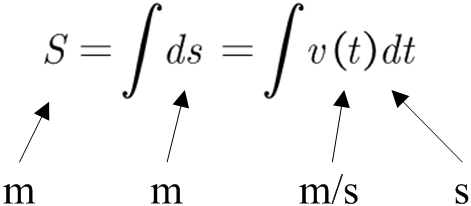
\includegraphics[height=2cm]{3.2.png}
% \end{figure}
所以,只要物理量是可以描述为加权积累效果的,都可以用定积分计算。




